%%%%%%%%%%%%%%%%%%%%%%%%%%%%%%%%%%%%%%%%%%%%%%%%%%%%%%%%%%%%%%%%%%%%%%%%%%%%%%%%
%          PLANTILLA DE TESIS — UNIVERSIDAD MICHOACANA DE SAN NICOLÁS
%                              DE HIDALGO (UMSNH)
%%%%%%%%%%%%%%%%%%%%%%%%%%%%%%%%%%%%%%%%%%%%%%%%%%%%%%%%%%%%%%%%%%%%%%%%%%%%%%%%
%  Formato FISMAT-UMSNH (clase PhDthesisPSnPDF, GNU GPL v3).
%  Plantilla genérica de ejemplo: sustituya TODOS los datos marcados
%  entre corchetes o con «Nombre...» / «Título...» por los suyos.
%  Cómo usarla: vea README.md

% openany: los capítulos empiezan en cualquier página (sin openany, la
% clase libro los fuerza a página impar y el PDF se llena de páginas en
% blanco). Para impresión a doble cara, quitar openany.
\documentclass[twoside,11pt,openany]{Latex/Classes/PhDthesisPSnPDF}
\usepackage{helvet}
%\renewcommand*\familydefault{\ttdefault} %% Solo si la fuente base será typewriter
\usepackage[T1]{fontenc}
\usepackage[spanish]{babel}

% Paquetes extra (pueden incluirse aquí o en la clase).
\usepackage{ragged2e}
\usepackage[square,sort,numbers]{natbib}
\usepackage{tikz} % Solo para la figura de ejemplo del capítulo 2
\usepackage{booktabs} % Reglas \toprule, \midrule y \bottomrule para las tablas

% This file contains macros that can be called up from connected TeX files
% It helps to summarise repeated code, e.g. figure insertion (see below).

%%%%%%%%%%%%%%%%%%%%%%%%%%%%%%%%%%%%%%%%%%%%%%
%            Colores de la UNAM              %
%%%%%%%%%%%%%%%%%%%%%%%%%%%%%%%%%%%%%%%%%%%%%%
%Azul Pantone 541  -->(0,63,119) RGB
\definecolor{Azul}{RGB}{0,63,119}

%Oro Pantone 460  -->(234,221,150) RGB
\definecolor{Oro}{RGB}{234,221,150}


%%%%%%%%%%%%%%%%%%%%%%%%%%%%%%%%%%%%%%%%%%%%%%
%            Comandos para líneas            %
%%%%%%%%%%%%%%%%%%%%%%%%%%%%%%%%%%%%%%%%%%%%%%
%Se define un comando \colorvrule para hacer líneas verticales de color con 3 argumentos: color, ancho, alto
\newcommand{\colorvrule}[3]{
\begingroup\color{#1}\vrule width#2 height#3
\endgroup}

%Se define un comando \colorhrule para hacer líneas horizontales de color con 2 argumentos: color, ancho
\newcommand{\colorhrule}[2]{
\begingroup\color{#1}\hrule height#2
\endgroup}

%%%%%%%%%%%%%%%%%%%%%%%%%%%%%%%%%%%%%%%%%%%%%%
%          Comando para derivadas            %
%%%%%%%%%%%%%%%%%%%%%%%%%%%%%%%%%%%%%%%%%%%%%%
\newcommand{\derivada}[3][]{\ensuremath{\dfrac{\mbox{d}^{#1}#2}{\mbox{d}#3^{#1}}}} 
%primer argumento(opcional): orden de la derivada
%segundo argumento: función a derivar
%tercer argumento: variable respecto a la que se deriva


%%%%%%%%%%%%%%%%%%%%%%%%%%%%%%%%%%%%%%%%%%%%%%
%       Comando para la exponencial          %
%%%%%%%%%%%%%%%%%%%%%%%%%%%%%%%%%%%%%%%%%%%%%%
\newcommand{\e}[1][]{\ensuremath{\mbox{e}^{#1}}}
%primer argumento(opcional): exponente de la exponencial




% insert a centered figure with caption and description
% parameters 1:filename, 2:title, 3:description and label
\newcommand{\figuremacro}[3]{
	\begin{figure}[htbp]
		\centering
		\includegraphics[width=1\textwidth]{#1}
		\caption[#2]{\textbf{#2} - #3}
		\label{condicion}
	\end{figure}
}

% insert a centered figure with caption and description AND WIDTH
% parameters 1:filename, 2:title, 3:description and label, 4: textwidth
% textwidth 1 means as text, 0.5 means half the width of the text
\newcommand{\figuremacroW}[4]{
	\begin{figure}[htbp]
		\centering
		\includegraphics[width=#4\textwidth]{#1}
		\caption[#2]{\textbf{#2} - #3}
		\label{#1}
	\end{figure}
}

% inserts a figure with wrapped around text; only suitable for NARROW figs
% o is for outside on a double paged document; others: l, r, i(inside)
% text and figure will each be half of the document width
% note: long captions often crash with adjacent content; take care
% in general: above 2 macro produce more reliable layout
\newcommand{\figuremacroN}[3]{
	\begin{wrapfigure}{o}{0.5\textwidth}
		\centering
		\includegraphics[width=0.48\textwidth]{#1}
		\caption[#2]{{\small\textbf{#2} - #3}}
		\label{#1}
	\end{wrapfigure}
}

% predefined commands by Harish
\newcommand{\PdfPsText}[2]{
  \ifpdf
     #1
  \else
     #2
  \fi
}

\newcommand{\IncludeGraphicsH}[3]{
  \PdfPsText{\includegraphics[height=#2]{#1}}{\includegraphics[bb = #3, height=#2]{#1}}
}

\newcommand{\IncludeGraphicsW}[3]{
  \PdfPsText{\includegraphics[width=#2]{#1}}{\includegraphics[bb = #3, width=#2]{#1}}
}

\newcommand{\InsertFig}[3]{
  \begin{figure}[!htbp]
    \begin{center}
      \leavevmode
      #1
      \caption{#2}
      \label{#3}
    \end{center}
  \end{figure}
}







%%% Local Variables:
%%% mode: latex
%%% TeX-master: "~/Documents/LaTeX/CUEDThesisPSnPDF/thesis"
%%% End:


%%%%%%%%%%%%%%%%%%%%%%%%%%%%%%%%%%%%%%%%%%%%%%%%%%%%%%%%%%%%%%%%%%%%%%%%%%%%%%%%
%                                   DATOS
%              (SUSTITUIR: son solo valores de ejemplo)
%%%%%%%%%%%%%%%%%%%%%%%%%%%%%%%%%%%%%%%%%%%%%%%%%%%%%%%%%%%%%%%%%%%%%%%%%%%%%%%%

\title{Título de la tesis}
\author{Nombre del Autor \\}
\facultad{Facultad de Ciencias Físico Matemáticas \\ ``Mat. Luis Manuel Rivera Gutiérrez''}

\escudofacultad{Latex/Classes/Escudos/logo_FISMAT}

\degree{Doctor en Ciencias en Ingeniería Física}
\director{Dr. Nombre del Director \\ Institución del director}
\matricula{[número de matrícula]}
\correo{[correo institucional]}
\degreedate{mes, año}
\lugar{Morelia, Michoacán, México}
\portadafalse

%% Comité tutor (descomentar y completar si aplica; si no hay codirector,
%% borre la línea siguiente: la portada lo imprime tal como está aquí).
\ctutoruno{Dr. Nombre del Codirector \\ Institución del codirector}

%% Opciones del posgrado (descomentar si las necesitan)
%\posgradotrue
%\programa{programa de maestría y doctorado en ingeniería}
%\campo{Ingeniería Eléctrica - Control}
%% Datos del jurado (descomentar y completar al entregar)
%\presidente{Dr. Nombre del Presidente}
%\secretario{Dr. Nombre del Secretario}
%\vocal{Dr. Nombre del Vocal}
%\supuno{Dr. Nombre del Primer Suplente}
%\supdos{Dr. Nombre del Segundo Suplente}
%\institucion{la institución donde se realizó la tesis}

\keywords{palabra clave 1, palabra clave 2, palabra clave 3}
\subject{tesis, plantilla}


%%%%%%%%%%%%%%%%%%%%%%%%%%%%%%%%%%%%%%%%%%%%%%%%%%%%%
%                   PORTADA
%%%%%%%%%%%%%%%%%%%%%%%%%%%%%%%%%%%%%%%%%%%%%%%%%%%%%
\begin{document}
% La portada se genera automáticamente desde los datos de arriba.
\maketitle

%%%%%%%%%%%%%%%%%%%%%%%%%%%%%%%%%%%%%%%%%%%%%%%%%%%%%
%                  PRÓLOGO
%%%%%%%%%%%%%%%%%%%%%%%%%%%%%%%%%%%%%%%%%%%%%%%%%%%%%
\frontmatter
{\Huge Declaración de Responsabilidad}
\newline
\newline

Declaro que esta tesis titulada ”Título de la tesis” es un trabajo original de mi investigación y ha sido escrita completamente por mí.

Declaro que este trabajo de tesis de investigación no constituye en ninguna de sus partes un plagio del trabajo material o intelectual de ningún otro autor.

Declaro que esta tesis es prácticamente en su totalidad producto de mi propio trabajo, la contribución colaborativa ha sido indicada claramente y reconocida.

Declaro que este trabajo de tesis no contiene material que haya sido aceptado o presentado para obtener cualquier otro grado académico, otro título o diploma en una universidad o cualquier otra institución de educación superior distinta a la Universidad Michoacana de San Nicolás de Hidalgo.

Declaro que se han proporcionado las debidas referencias sobre toda la literatura y los recursos de apoyo, respetando íntegramente el contenido científico de los trabajos aquí citados, y que la presente tesis es original en su totalidad y no se deriva de ningún otro trabajo citado.

\vspace{10mm}

Autor

\vspace{15mm}

Nombre del Autor

\vspace{15mm}

Asesor

\vspace{15mm}

Dr. Nombre del Director

\begin{dedication}
[Texto de dedicatoria de ejemplo. Sustitúyalo por su dedicatoria, o elimine
este archivo y su llamada en el documento principal.]
\end{dedication}

\begin{acknowledgements}
[Texto de agradecimientos de ejemplo. Agradezca aquí a las personas e
instituciones que apoyaron el desarrollo de su trabajo.]

Plantilla elaborada a partir del formato FISMAT-UMSNH y compartida por Reox Lab --- reoxlab.com
\end{acknowledgements}

%\begin{abstractslong}    %uncommenting this line, gives a different abstract heading
\begin{resumen}

Este es el resumen de ejemplo de la plantilla. Escriba aquí, en un máximo
de una página, el objetivo del trabajo, la metodología empleada, los
resultados principales y las conclusiones.

\vfill
\textbf{Palabras clave:} palabra clave 1, palabra clave 2, palabra clave 3.
\end{resumen}
%\end{abstractlongs}

\begin{abstracts}

This is the example abstract of the template. Write here, in no more than
one page, the objective of the work, the methodology, the main results and
the conclusions.

\vfill

\textbf{Keywords:} keyword 1, keyword 2, keyword 3.
\end{abstracts}
%\end{abstractlongs}


%%%%%%%%%%%%%%%%%%%%%%%%%%%%%%%%%%%%%%%%%%%%%%%%%%%%%
%                   ÍNDICES
%%%%%%%%%%%%%%%%%%%%%%%%%%%%%%%%%%%%%%%%%%%%%%%%%%%%%

% Esta sección genera el índice
\setcounter{secnumdepth}{3} % nivel que recibe numeración
\setcounter{tocdepth}{3}    % nivel que se imprime en el índice
\tableofcontents            % Genera el índice
%: ----------------------- list of figures/tables ------------------------
%\listoffigures              % Genera el índice de figuras (descomentar si se usa)
%\listoftables               % Genera el índice de tablas (descomentar si se usa)


%%%%%%%%%%%%%%%%%%%%%%%%%%%%%%%%%%%%%%%%%%%%%%%%%%%%%
%                   CONTENIDO
%%%%%%%%%%%%%%%%%%%%%%%%%%%%%%%%%%%%%%%%%%%%%%%%%%%%%
\mainmatter
% Interlineado de 1.5
\def\baselinestretch{1.5}
\chapter{Introducción}\label{Chap1}

\epigraph{ \emph{``El conocimiento es poder.''}}{--- \textup{Francis Bacon}}

\section{Motivación y contexto general}

[Texto de ejemplo. Escriba aquí por qué importa el problema de su tesis,
en qué contexto se inscribe y qué se ha hecho antes sobre él. Dos o tres
párrafos bastan para esta sección.]

\section{Objetivos de la tesis}

\subsection{Objetivo general}

[Texto de ejemplo. Escriba aquí el objetivo general de la tesis en una o
dos frases.]

\subsection{Objetivos específicos}

[Texto de ejemplo. Enumere aquí los objetivos específicos:]
\begin{itemize}
\item Primer objetivo específico de ejemplo.
\item Segundo objetivo específico de ejemplo.
\item Tercer objetivo específico de ejemplo.
\end{itemize}

\section{Organización de la tesis}

[Texto de ejemplo. Describa brevemente el contenido del capítulo 2 y del
apéndice A, para que el lector sepa qué encontrará en cada parte.]

\chapter{Desarrollo}\label{Chap2}

\section{Marco teórico}

[Texto de ejemplo. Presente aquí los conceptos y definiciones necesarios
para entender el trabajo. Cada ecuación debe ir seguida de la definición
de sus símbolos, como en el ejemplo siguiente.]

\begin{equation}
y = ax^2 + bx + c
\label{eq:ejemplo}
\end{equation}

donde $y$ es la variable dependiente, $x$ es la variable independiente, y
$a$, $b$ y $c$ son coeficientes constantes. La ecuación~\eqref{eq:ejemplo}
se cita en el texto con su número, así: la ecuación~\eqref{eq:ejemplo}
describe una parábola.

\section{Metodología}

[Texto de ejemplo. Describa aquí cómo se realizó el trabajo: métodos,
materiales y procedimiento. Los conceptos de \cite{libro-ejemplo} sirven
de referencia para esta sección.]

\begin{figure}[htbp]
	\centering
	\begin{tikzpicture}[scale=0.9]
		\draw[->] (-2.5,0) -- (2.5,0) node[right] {$x$};
		\draw[->] (0,-0.5) -- (0,4.5) node[above] {$y$};
		\draw[domain=-2:2,smooth,variable=\x,thick] plot ({\x},{\x*\x});
	\end{tikzpicture}
	\caption[Figura de ejemplo]{Figura de ejemplo: parábola $y = x^2$.}
	\label{fig:ejemplo}
\end{figure}

La figura~\ref{fig:ejemplo} muestra un ejemplo de figura con su pie y su
etiqueta: toda figura debe introducirse y comentarse en el texto.

\section{Resultados de ejemplo}

[Texto de ejemplo. Presente aquí los resultados principales y compárelos
con lo reportado en la literatura, por ejemplo en
\cite{articulo-ejemplo}.]

\begin{table}[htbp]
	\centering
	\caption[Tabla de ejemplo]{Tabla de ejemplo: datos ilustrativos.}
	\label{tab:ejemplo}
	\begin{tabular}{lcc}
	\hline
	Caso & Valor A & Valor B \\
	\hline
	1 & 1.0 & 2.0 \\
	2 & 1.5 & 2.5 \\
	3 & 2.0 & 3.0 \\
	\hline
	\end{tabular}
\end{table}

La tabla~\ref{tab:ejemplo} resume los datos de ejemplo: toda tabla debe
introducirse y comentarse en el texto, igual que las figuras.

\chapter{Mini tutorial de LaTeX}\label{ChapTutorial}

[Este capítulo es un tutorial breve: cada sección muestra un recurso
básico de LaTeX con un ejemplo que compila. Borre este capítulo cuando su
tesis esté lista, o consérvelo como referencia. Lo que aquí se ejemplifica
—listas, ecuaciones, letras griegas, citas, figuras y tablas— es lo que
más se usa al escribir una tesis.]

\section{Estructura: capítulos, secciones y referencias cruzadas}

Un documento se divide en \verb|\chapter|, \verb|\section| y
\verb|\subsection|. Para referirse a otra parte del documento se pone una
etiqueta con \verb|\label| y se cita con \verb|\ref|. Por ejemplo, este
capítulo es el capítulo~\ref{ChapTutorial}, y la
sección~\ref{sec:ecuaciones} trata de ecuaciones. Las notas al pie se
hacen con \verb|\footnote|, como esta.\footnote{Esto es una nota al pie
de ejemplo. Sirve para aclaraciones que no caben en el texto principal.}

\section{Listas}

Hay tres tipos de lista. La lista sin orden usa \verb|itemize|:

\begin{itemize}
\item Primer elemento de la lista.
\item Segundo elemento de la lista.
\item Tercer elemento de la lista.
\end{itemize}

La lista numerada usa \verb|enumerate|:

\begin{enumerate}
\item Primer paso del procedimiento.
\item Segundo paso del procedimiento.
\item Tercer paso del procedimiento.
\end{enumerate}

La lista de descripción usa \verb|description|:

\begin{description}
\item[Concepto] Descripción breve del concepto.
\item[Método] Descripción breve del método.
\end{description}

\section{Ecuaciones}\label{sec:ecuaciones}

Una ecuación en línea se escribe entre signos de dólar: la energía es
$E = mc^2$, donde $E$ es la energía, $m$ es la masa y $c$ es la velocidad
de la luz. Una ecuación centrada y numerada usa el entorno
\verb|equation|:

\begin{equation}
E = mc^2
\label{eq:energia}
\end{equation}

donde $E$ es la energía, $m$ es la masa y $c$ es la velocidad de la luz.
La ecuación~\eqref{eq:energia} se cita con \verb|\eqref|. Para varias
ecuaciones alineadas por el signo igual se usa \verb|align| (del paquete
\verb|amsmath|, ya cargado por la clase):

\begin{align}
a^2 + b^2 &= c^2 \\
x &= \frac{-b \pm \sqrt{b^2 - 4ac}}{2a}
\label{eq:cuadratica}
\end{align}

donde $a$, $b$ y $c$ son coeficientes constantes. La
ecuación~\eqref{eq:cuadratica} es la fórmula general de segundo grado.

\section{Letras griegas}

Las letras griegas se escriben en modo matemático con su nombre en
inglés precedido de una barra invertida. La tabla~\ref{tab:griegas}
muestra las más usadas.

\begin{table}[htbp]
\centering
\caption[Letras griegas de ejemplo]{Letras griegas más usadas.}
\label{tab:griegas}
\begin{tabular}{lll}
\toprule
Nombre & Minúscula & Mayúscula \\
\midrule
alfa & $\alpha$ & --- \\
beta & $\beta$ & --- \\
gamma & $\gamma$ & $\Gamma$ \\
delta & $\delta$ & $\Delta$ \\
pi & $\pi$ & $\Pi$ \\
omega & $\omega$ & $\Omega$ \\
lambda & $\lambda$ & $\Lambda$ \\
mu & $\mu$ & --- \\
sigma & $\sigma$ & $\Sigma$ \\
\bottomrule
\end{tabular}
\end{table}

Por ejemplo, la constante $\pi$ vale aproximadamente $3.1416$, y un
incremento se escribe $\Delta x$. Las mayúsculas que coinciden con el
alfabeto latino (como la A de alfa) no tienen comando propio: se escriben
directamente.

\section{Citas bibliográficas}

Las referencias se guardan en el archivo \verb|.bib| y se citan con
\verb|\cite|. Por ejemplo, para un libro se escribe
\verb|\cite{libro-ejemplo}|, que produce \cite{libro-ejemplo}; para un
artículo, \verb|\cite{articulo-ejemplo}|, que produce
\cite{articulo-ejemplo}; y para un sitio web,
\verb|\cite{sitio-ejemplo}|, que produce \cite{sitio-ejemplo}. Con
\verb|natbib| (ya cargado por la plantilla) también se puede citar el
autor en el texto con \verb|\citet{libro-ejemplo}|:
\citet{libro-ejemplo} es un libro de ejemplo. Al final del documento, el
comando \verb|\bibliography| genera la lista con el estilo elegido en
\verb|\bibliographystyle|.

\section{Figuras}

Una figura se incluye con \verb|\includegraphics| dentro de un entorno
\verb|figure|, siempre con pie (\verb|\caption|) y etiqueta
(\verb|\label|) para citarla en el texto. La
figura~\ref{fig:escudo-ejemplo} muestra cómo incluir una imagen externa.

\begin{figure}[htbp]
\centering
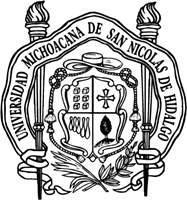
\includegraphics[width=0.25\textwidth]{Latex/Classes/Escudos/UMSNH_BN}
\caption[Ejemplo de imagen externa]{Ejemplo de imagen externa: escudo
de la UMSNH incluido con \texttt{\textbackslash includegraphics}.}
\label{fig:escudo-ejemplo}
\end{figure}

También se pueden dibujar figuras directamente en LaTeX con TikZ, como
la parábola del capítulo~\ref{Chap2}. El ancho se controla con
\verb|width|: \verb|0.25\textwidth| es un cuarto del ancho del texto.

\section{Tablas}

Una tabla se hace con el entorno \verb|tabular| dentro de \verb|table|,
con pie y etiqueta, igual que las figuras. Para tablas con mejor aspecto
se usa el paquete \verb|booktabs|, con las reglas \verb|\toprule|,
\verb|\midrule| y \verb|\bottomrule| en lugar de \verb|\hline| (véase la
tabla~\ref{tab:griegas}). La tabla~\ref{tab:ejemplo} del
capítulo~\ref{Chap2} muestra la versión sencilla con \verb|\hline|.

\section{Cómo compilar}

La forma recomendada es \verb|latexmk|, que repite las pasadas
necesarias (incluida la bibliografía) automáticamente:

\begin{verbatim}
latexmk -pdf plantilla-tesis-umsnh.tex
\end{verbatim}

Sin \verb|latexmk|, a mano (tres pasadas de \verb|pdflatex| con
\verb|bibtex| en medio):

\begin{verbatim}
pdflatex plantilla-tesis-umsnh.tex
bibtex plantilla-tesis-umsnh
pdflatex plantilla-tesis-umsnh.tex
pdflatex plantilla-tesis-umsnh.tex
\end{verbatim}

El PDF resultante no se versiona: se genera al compilar. Para limpiar
los archivos intermedios, use \verb|latexmk -c|.


%%%%%%%%%%%%%%%%%%%%%%%%%%%%%%%%%%%%%%%%%%%%%%%%%%%%%
%                   APÉNDICES
%%%%%%%%%%%%%%%%%%%%%%%%%%%%%%%%%%%%%%%%%%%%%%%%%%%%%
\appendix
\chapter{Apéndice de ejemplo}\label{ape:ejemplo}

[Texto de ejemplo. Los apéndices contienen el material complementario que
no cabe en los capítulos: deducciones largas, tablas extensas o código.
Cada apéndice es un capítulo más, con sus propias secciones.]

\section{Sección de ejemplo}

[Texto de ejemplo. Para más información sobre este tipo de recursos, véase
\cite{sitio-ejemplo}.]


%%%%%%%%%%%%%%%%%%%%%%%%%%%%%%%%%%%%%%%%%%%%%%%%%%%%%
%                   REFERENCIAS
%%%%%%%%%%%%%%%%%%%%%%%%%%%%%%%%%%%%%%%%%%%%%%%%%%%%%
% Existen varios estilos de bibliografía; pueden cambiarlos a placer.
\bibliographystyle{plainnat} % otros: abbrv, acm, alpha, apalike, ieeetr, plain, siam, unsrt

\bibliography{biblio/referencias-ejemplo} % Archivo .bib


\end{document}
